\begin{savequote}[75mm]
În comunitatea Python, a spune despre ceva că este isteț, \emph{nu} este considerat un compliment.
\qauthor{Alex Martelli}
\end{savequote}

\chapter{Python și Django}

În scurta mea carieră de inginer software, am lucrat deja cu trei limbaje de programare:
\emph{C\#}, \emph{Scala} și \emph{Python}. În acest capitol voi explica de ce am
ales Python pentru dezvoltarea back-end-ului acestui proiect.

\section{Python}

Python este un limbaj dinamic, interpretat care pune accent pe lizibilitate.

Avantaje:
\begin{itemize}
\item Foarte ușor de învățat și folosit, poți deveni productiv în doar câteva zile.
\item Comunitate puternică, deci se găsesc cu ușurință o mulțime de librării și framework-uri bine scrise și bine documentate și soluții la problemele comune.
\item Comunitatea și filosofia\footnote{Vezi Figura \ref{fig:zen}} limbajului au pus mare accent pe lizibilitatea codului.
Codul Python este foarte ușor de înțeles, chiar și de cineva fără experiență
cu acest limbaj, iar limbajul permite scrierea codului într-un mod elegant, concis și expresiv.
\end{itemize}

Dezavantaje:
\begin{itemize}
\item Fiind un limbaj dinamic, IDE-ul nu înțelege la fel de bine structura codului, iar refactorizările se fac mai greu decât în limbajele statice.
\item Este mai încet decât limbajele compilate.
\end{itemize}

În continuare, pentru comparare, prezint codul sursă al unui \emph{web crawler}\footnote{\url{http://en.wikipedia.org/wiki/Web\_crawler}}
foarte simplu, scris mai întâi în Java, apoi în Python. Codul este inspirat
din \emph{Java vs Python Platforms Comparison}, ce poate fi văzut la \url{https://www.youtube.com/watch?v=ppspz2ZiBaY}.

\begin{figure}
  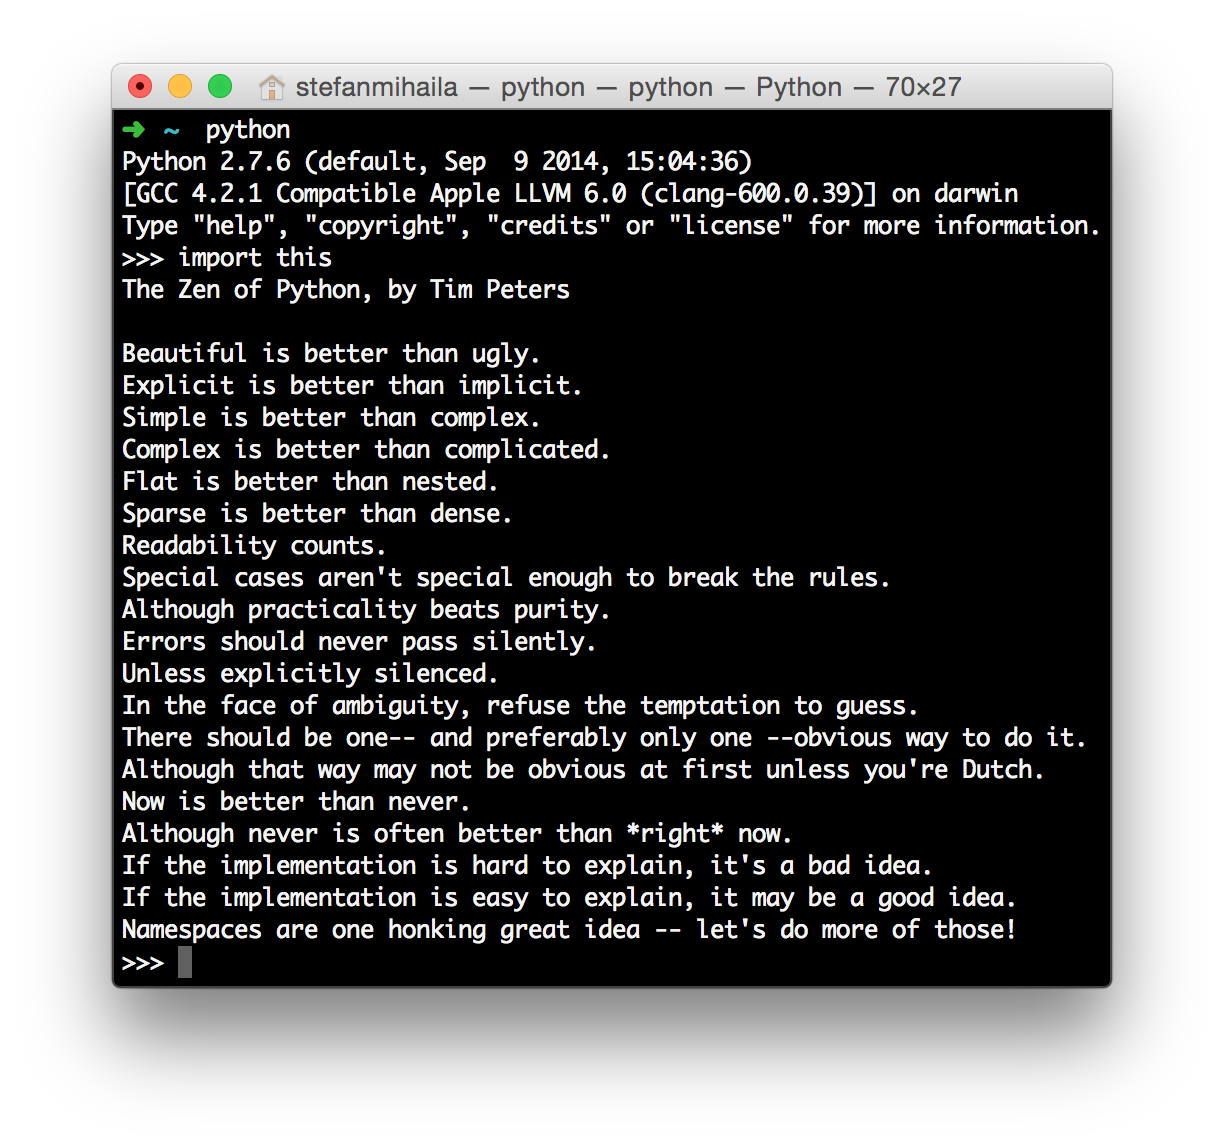
\includegraphics[width=1\textwidth]{./zen}
  \caption{The Zen of Python}
  \label{fig:zen}
\end{figure}

\lstinputlisting[language=Java, title=\lstname]{Main.java}

Iar acum, varianta Python:
\lstinputlisting[language=Python, title=\lstname]{crawler.py}

Ambele programe fac același lucru: primesc un URL de la utilizator, cer pagina
aflată la acel URL și folosesc o expresie regulată pentru a găsi toate link-urile
din pagina respectivă. Totuși, se poate observa că varianta scrisă în Python
este mai scurtă și mai ușor de înțeles.


\section{Django}

\emph{Django} este un framework web implementat în Python. Motto-ul lui este: 
"Un framework pentru perfecționiștii cu termene limită".

Django poate fi considerat un framework MVC, dar folosește o terminologie proprie:
\begin{itemize}
\item \emph{Modelul} este reprezentat de ORM-ul (Object-relational mapping)\footnote{\url{http://en.wikipedia.org/wiki/Object-relational\_mapping}} framework-ului care face legătura dintre obiecte Python și tabele dintr-o bază de date relațională.
\item Clasele sau funcțiile care creeză răspunsul la request sunt denumite \emph{view}-uri. Acestea sunt denumite \emph{controller}-ere în alte framework-uri MVC.
\item Datele sunt prezentate folosind șabloane (templates). Acestea sunt ceea ce alte framework-uri numesc \emph{view}-uri.
\item \emph{Controller}-ul este reprezentat de însuși framework, care rutează
un request la view-ul corespunzător URL-ului cerut (prin URL dispatcher).
\end{itemize}
